\documentclass{isprs} 

\usepackage{subfigure}
\usepackage{setspace}
\usepackage{geometry}
\usepackage[labelsep=period]{caption}  
\usepackage[british]{babel} 

%\usepackage{natbib}
\usepackage{amsfonts,amsmath,bm,bbm}
\usepackage{hyperref} 
\usepackage{graphicx,xurl}
\usepackage{rotating}
\usepackage{todonotes}
\usepackage{lipsum}
\usepackage{xcolor}

\usepackage{tikz}
\usepackage{ifthen}

\geometry{a4paper, top=25mm, left=20mm, right=20mm, bottom=25mm, headsep=10mm, footskip=12mm}

\captionsetup{justification=centering,font=normal} 
\captionsetup[figure]{font=small}

\usepackage{color}

\hyphenation{}

\newdimen\HilbertLastX
\newdimen\HilbertLastY
\newcounter{HilbertOrder}

\def\DrawToNext#1#2{%
   \advance \HilbertLastX by #1
   \advance \HilbertLastY by #2
   \pgfpathlineto{\pgfqpoint{\HilbertLastX}{\HilbertLastY}}
   % Alternative implementation using plot streams:
   % \pgfplotstreampoint{\pgfqpoint{\HilbertLastX}{\HilbertLastY}}
}

% \Hilbert[right_x,right_y,left_x,left_x,up_x,up_y,down_x,down_y]
\def\Hilbert[#1,#2,#3,#4,#5,#6,#7,#8] {
  \ifnum\value{HilbertOrder} > 0%
     \addtocounter{HilbertOrder}{-1}
     \Hilbert[#5,#6,#7,#8,#1,#2,#3,#4]
     \DrawToNext {#1} {#2}
     \Hilbert[#1,#2,#3,#4,#5,#6,#7,#8]
     \DrawToNext {#5} {#6}
     \Hilbert[#1,#2,#3,#4,#5,#6,#7,#8]
     \DrawToNext {#3} {#4}
     \Hilbert[#7,#8,#5,#6,#3,#4,#1,#2]
     \addtocounter{HilbertOrder}{1}
  \fi
}

% \hilbert((x,y),order)
\def\hilbert((#1,#2),#3){%
   \advance \HilbertLastX by #1
   \advance \HilbertLastY by #2
   \pgfpathmoveto{\pgfqpoint{\HilbertLastX}{\HilbertLastY}}
   % Alternative implementation using plot streams:
   % \pgfplothandlerlineto
   % \pgfplotstreamstart
   % \pgfplotstreampoint{\pgfqpoint{\HilbertLastX}{\HilbertLastY}}
   \setcounter{HilbertOrder}{#3}
   \Hilbert[1mm,0mm,-1mm,0mm,0mm,1mm,0mm,-1mm]
   \pgfusepath{stroke}%
}

\begin{document}

\title{CHARACTERIZATION OF SAR IMAGES WITH WEIGHTED AMPLITUDE TRANSITION GRAPHS}

\author{
	Eduarda T.\ C.\ Chagas\textsuperscript{1}, 
	Alejandro C.\ Frery\textsuperscript{2}\thanks{Corresponding author},
	Osvaldo A.\ Rosso\textsuperscript{3},
	Heitor S.\ Ramos\textsuperscript{1}
}

\address{
	\textsuperscript{1 }Dept.\ de Ci\^encia da Computa\c c\~ao, Universidade Federal de Minas Gerais, Belo Horizonte, Minas Gerais, Brazil\\ (eduarda.chagas, ramosh)@dcc.ufmg.br,\\
	\textsuperscript{2 } Laborat\'orio de Computa\c c\~ao Cient\'ifica e An\'alise Num\'erica -- LaCCAN, Universidade Federal de Alagoas, Brasil \\ acfrery@laccan.ufal.br\\
	\textsuperscript{3 }Instituto de F\'isica, Universidade Federal de Alagoas, Brasil,\\
	Instituto de Medicina Traslacional e Ingenier\'ia Biom\'edica\\
	Hospital Italiano de Buenos Aires \& Conicet, Argentina \\
	oarosso@if.ufal.br
}

\icwg{}   

\abstract{
	We propose a new technique for SAR image texture characterization based on ordinal pattern transition graphs.
	The proposal consists in
	(i)~transforming a 2-D patch of data into a time series using a Hilbert Space Filling Curve,
	(ii)~building an Ordinal Pattern Transition Graph with weighted edges;
	(iii)~obtaining a probability distribution function from this graph;
	(iv)~computing the Entropy and Statistical Complexity of this distribution.
	The weight of the edges is related to the absolute difference of observations.
	This modification takes into account the scattering properties of the target, and leads to a good characterization of several types of textures.
	Experiments with data from Munich urban areas, Guatemala forest regions, and Cape Canaveral ocean samples demonstrate the effectiveness of our technique, which achieves satisfactory levels of separability.
}


\keywords{Synthetic Aperture Radar (SAR), Time-series, Terrain Classification, Permutation Entropy, Ordinal Patterns Transition Graphs, Causality Complexity-Entropy Plane.}

\maketitle

\section{INTRODUCTION}\label{Intro}

Surface classification and land use are among the most important applications of Synthetic Aperture Radar (SAR) imaging \cite{Pottier2004Unsupervised}, for which supervised and unsupervised classification algorithms have been proposed~\cite{han2020unsupervised,huang2020classification,xie2020polsar}.

Classification techniques rely on the extraction and analysis of features from the data, and from additional information and prior knowledge about  the scene, the sensor and the acquisition conditions.
Texture is among the features that carries most information and, as such, it is important to characterize it in a quantitative manner.

The texture in SAR images is characterized twofold, namely by the marginal properties of the data, and by their spatial structure~\cite{numbisi2018multi}.
In this work we focus on the second approach.

The most widely used approach to obtain textural features from SAR imagery is through co-ocurrence matrices and Haralick's descriptors~\cite{yu2019detection}.
Other approaches include the Fourier power spectrum~\cite{Florindo2012Fractal}, and
random fields~\cite{zhu2016antarctic}.

In our approach, we opt to linearize the image patches and analyze the resultant 1-D signals as time series. 
By doing that, we reduce the dimensionality of the data and map spatial dependence of pixels to temporal correlation. 
Then, we extract ordinal patterns from the time series and propose a novel weighted graph of pattern transitions that is able to discriminate patterns correspondent to different amplitude levels. 
We then used well-known features from information theory to characterize the image patches. 
	
The main contribution of this work is the proposal of a novel technique for SAR image texture characterization that is based on a modified version of ordinal pattern transition graphs, which is able to discriminate similar patterns with different amplitude levels. 
Our approach yields to interesting characterization of several types of textures as shown in experiments with real data achieving satisfactory levels of separability.

The article was divided as follows:
Section~\ref{methodology} presents the proposed methodology.
Section~\ref{linearization} reports how the patch linearization process of the images occurs.
Section~\ref{WATG} describes our technique of ordinal amplitude transition graph weighting by amplitudes.
In Section~\ref{HC} we report the Information Theory descriptors used throughout this work.
Section~\ref{SAR} shows the results obtained in characterizing textures.
We present our conclusions in Section~\ref{Conclusion}.


\section{Methodology}\label{methodology}

Our procedure consists of the following steps:
\begin{enumerate}
	\item\label{item:Linearlize} transforming a 2-D patch of data into a time series using a Hilbert Space Filling Curve,
	\item\label{item:WOPTG} building an Ordinal Pattern Transition Graph with weighted edges;
	\item\label{item:Probability} obtaining a probability distribution function from this graph;
	\item\label{item:Descriptors} computing the Entropy and Statistical Complexity of this distribution.
\end{enumerate}
The technique is illustrated in Figure~\ref{fig:WATG}, and detailed in the following.

	
\begin{figure}[hbt]
	\centering
	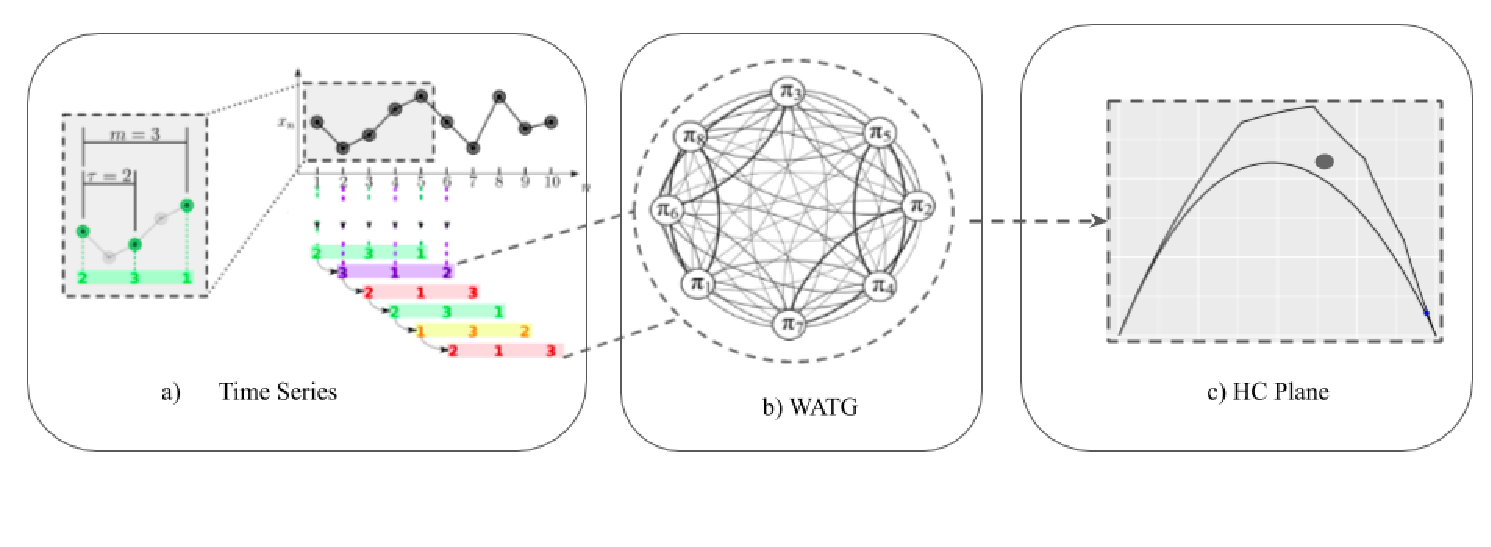
\includegraphics[scale = 0.32]{Figures/WATG.pdf}
	%\vspace{-1.2cm}
	\caption{Outline of the technique for the characterization of textures.}
	\label{fig:WATG}
\end{figure}

\subsection{Linearization of image patches}\label{linearization}

In this step, we perform a data dimensionality reduction by turning 2-D patches into 1-D signals.
For this, we opt to do a linearization of the data through techniques that maintain the spatial correlation of the image.
This could be accomplished by reading the data by lines, columns or any transformation.
In Step~\ref{item:Linearlize} we employ a Hilbert Space Filling Curve~\cite{Lee1994Texture}.

Space filling curves were first employed by Nguyen and Quinqueton (1982), to map a texture into a one-dimensional signal.
When used as scanning methods of an image, such functions preserve relevant properties of pixel spatial correlation~\cite{Lee1994Texture}.

Assuming an image patch is supported by a $N \times N$ dimension grid, where $N$ is a power of $2$, we have the following definition.

\newtheorem{mydef}{Definition}
\begin{mydef}
	An image scan is a bijective function $f \colon \mathbb{N} \times \mathbb{N} \to \mathbb{N}$ in the ordered pair set $ \{(i, j): 1 \leq i , j \leq N \}$, which denotes the points in the domain, for the closed range of integers $\{1, \dots, N^2\}$.
	A scan rule is $\{f^{-1}(1), \dots, f^{-1}(N^2)\}$.
	\label{def:CurveFilling}
\end{mydef}
This Definition imposes that each pixel is visited only once.

Space filling curves, such as raster-1, raster-2 and Hilbert scanning techniques stipulate a proper function $f$.
Hilbert curves scans an array of pixels of dimension $2^k \times 2^k$, $k \in \mathbb{N}$, never keeping the same direction for more than three consecutive points, as shown in Figure~\ref{fig:Hilbert}.
Using the Hilbert curve, we can reduce the data dimensionality by maintaining the spatial dependence information of the analyzed textures.
In this work, we use only a Hilbert Curves scale in images of dimension $128 \times 128$.


\begin{figure}[hbt]
	\centering
	\tikz[scale=2.6] \hilbert((0mm,0mm),3);
	\hspace{0.3cm}
	\tikz[scale=1.2] \hilbert((0mm,0mm),4);
	\hspace{0.3cm}
	\tikz[scale=0.58] \hilbert((0mm,0mm),5);	
	\caption{Hilbert space filling curve in areas of: (a) $8 \times 8$, (b) $16 \times 16$ and (c) $32 \times 32$. }\label{fig:Hilbert}
\end{figure} 

\subsection{Weighted Ordinal Patterns Transition Graph}\label{WATG}

Step~\ref{item:WOPTG} consists of two stages.
In the first, the time series is transformed into a sequence of ordinal patterns.
In the second, we build a weighted graph describing the transitions between these patterns.

The representation of time series by ordinal patterns was introduced by~\cite{Bandt2002Permutation} as a transformation resistant to noise, and invariant to nonlinear monotonic transformations.

Consider ${\mathcal X} \equiv \{x_t\}_{t=1}^{T}$ a real valued time series of length $T$. 

Let ${\mathfrak A}_{D}$ (with $D \geq 2$ and $D \in {\Bbb N}$) be the symmetric group of order $D!$ formed by all 
possible permutation of order $D$, and the symbol component vector 
${\bm \pi}^{(D)} = (\pi_1, \pi_2, \dots, \pi_D)$ so every element ${\bm \pi}^{(D)}$ is unique 
($\pi_j \neq \pi_k$ for every $j \neq k$). 
Consider for the time series ${\mathcal X} \equiv \{x_t\}_{t=1}^{T}$ its time delay embedding representation,
with embedding dimension $D \geq 2$ and time delay $\tau \geq 1$ ($\tau \in {\Bbb N}$, also called ``embedding time'', ``time delay'', or ``delay''):

\begin{equation} 
\label{eq:time-delay}
{\mathbf X}^{(D,\tau)}_t ~=~( x_t,x_{t+\tau},\dots,x_{t+(D-1)\tau} ) ,
\end{equation} 

for $t = 1,2,\dots,N$ with $N = T-(D-1) \tau$.
Then the vector ${\mathbf X}^{(D,\tau)}_t$ can be mapped to a symbol vector ${\bm \pi}_t^D \in {\mathfrak A}_{D}$. 
This mapping should be defined in a way that preserves the desired relation between the elements 
$x_t  \in {\mathbf X}^{(D,\tau)}_t$, and all $t \in \{1,\dots,T-(D-1)\tau\}$ that share this pattern (also called ``motif'') have to mapped to the same 
${\bm \pi}_t^{D}$.

We define the mapping ${\mathbf X}_t^{(D,\tau)} \mapsto {\mathbf \pi}_t^{D}$ by ordering the observations $x_t \in {\mathbf X}_t^{(D,\tau)}$ in increasing order.
Consider the time series $\mathcal X = (1.8, 1.2, 3.2, 4.8, 4.2, 4.5, 2.3, 3.7, 1.2, .5)$ depicted in Fig.~\ref{Fig:IntroBP}.
Assume we are using patterns of length $D=5$ with unitary time lag $\tau=1$.
The code associated to $\mathbf X_{3}^{(5,1)}=(x_3,\dots,x_7)=(3.2, 4.8, 4.2, 4.5, 2.3)$, shown in black, is formed by the indexes in $\bm\pi_3^{5}=(1,2,3,4,5)$ which sort the elements of $\mathbf X_{3}^{(5,1)}$ in increasing order: $51342$.
With this, $\widetilde{\pi}_3^{5} = 51342$, and we increase the counting related to this motif in the histogram of all possible patterns of size $D=5$.

The dash-dot line in Fig.~\ref{Fig:IntroBP} illustrates $\mathbf X_{1}^{(5,2)}$, i.e. the sequence of length $D=5$ starting at $x_1$ with lag $\tau=2$.
In this case, $\mathbf X_{1}^{(5,2)}= (1.8, 3.2, 4.2, 2.3, 1.2)$, and the corresponding motif is $\widetilde{\pi}_1^{5}=51423$.

\begin{figure}[hbt]
	\centering
	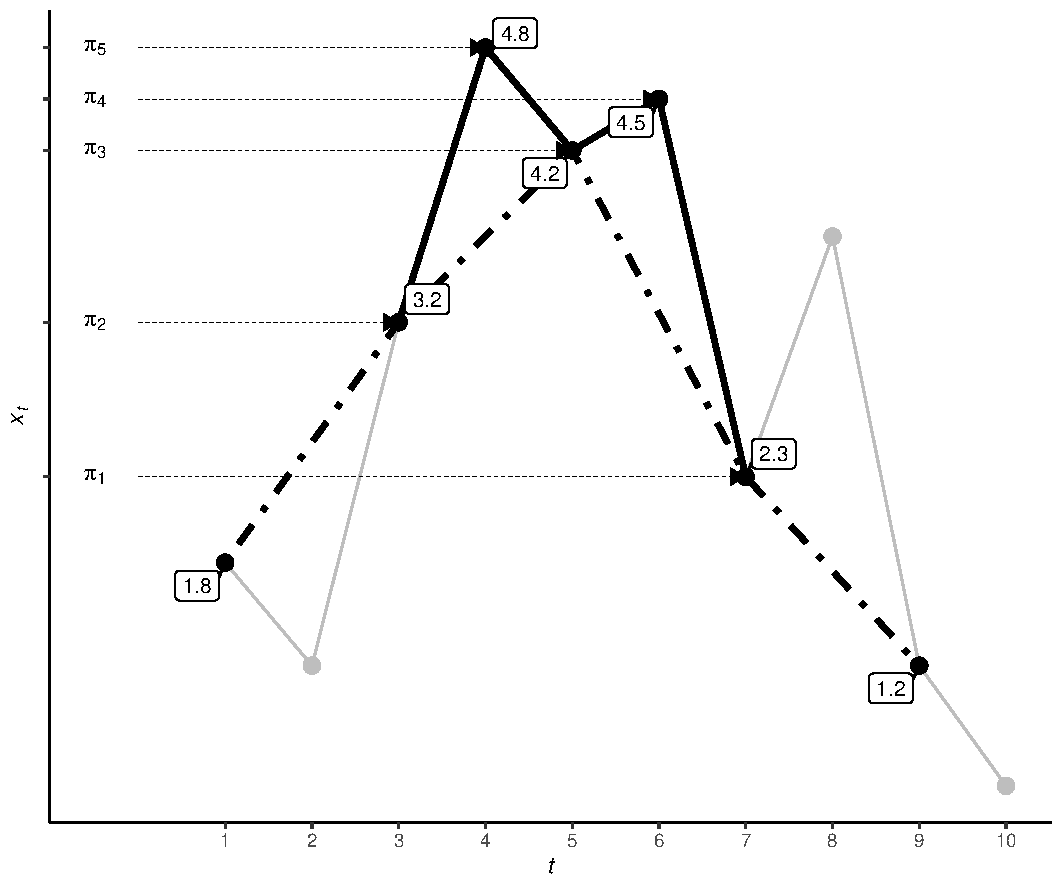
\includegraphics[width=.9\linewidth]{../../Figures/IntroBP.pdf}
	\caption{Illustration of the Bandt and Pompe coding\label{Fig:IntroBP}}
\end{figure}

The classical approach consists in analyzing the histogram of these patterns.
Alternatively, one may form an oriented graph with the transitions from $\widetilde\pi_t^D$ to $\widetilde\pi_{t+1}^D$.
We modify this last approach by assigning weights to the edges related to the absolute difference of the observations.
This modification takes into account the scattering properties of the target, and leads to a good characterization of several types of textures.

Denote $\Pi$ the sequence of symbols obtained by a given series $\mathbf{X}_t^{(D,\tau)}$.
The Bandt-Pompe probability distribution is the relative frequency of symbols in the series against $D!$ possible permutations of patterns $\{\widetilde\pi_t^D \}_{t = 1}^{D!}$:
\begin{equation}
p(\widetilde\pi_t^D) = \frac{\#\left \{t : t = 1, \dots, T-(D-1)\tau; \mathbf{X}_t^{(D,\tau)} \text{ is of type } \widetilde\pi_t^D\right \}}{T- (D-1)\tau},  
\end{equation}
that meets the conditions $p(\widetilde\pi_t^D) \ge 0$ and  $\sum_{i=1}^{D!} p(\widetilde\pi_t^D) = 1$.

The Ordinal Pattern Transition Graph ${G} = ({V}, {E})$ 
represents the transitions between two consecutive ordinal patterns over time $t$.
The vertices are the patterns, and the edges the transitions between them:
$V = \{v_{\widetilde\pi_t^D}\}$, and 
$E = \{(v_{\widetilde\pi_t^D}, v_{\widetilde\pi_{t+1}^D}): v_{\widetilde\pi_t^D}, v_{\widetilde\pi_{t+1}^D} \in V \}$~\cite{LearningandDistinguishingTimeSeriesDynamicsViaOrdinalPatternsTransitionGraphs2019}.

Recent works propose a weighting in the calculation of relative frequencies for ordinal patterns with different amplitude variances, making them contribute differently to the final value of permutation entropy (PE) and thus incorporating amplitude change information within a given set~\cite{Fadlallah2013Weightedpermutation}.
However, these methods do not consider the amplitude difference present in different time series, weighing them similarly when calculating the final value of their probabilities.
Therefore, data with different amplitudes but with similar variance dynamics are not discriminated, losing important information about the system dynamics.

To counterbalance these facts, we propose a modification of the current ordinal pattern transition graph by incorporating meaningful time series information.

Two approaches are considered in relation to the weight of edges in the literature.
Some authors employ unweighted edge~\cite{McCullough2015lagged,Kulp2016ordinal} representing only the existence of such transitions, while others apply the frequency of transitions~\cite{Sorrentino2015periodic,Zhang2017ConstructingOP}.
The weights $\mathbb{W} = \{w_{v_{\widetilde{\pi}^D_i}, v_{\widetilde\pi^D_j}}: v_{\widetilde\pi^D_i}, v_{\widetilde\pi^D_j} \in V \}$ assigned to each edge describes the chances of transition between two particular patterns $(v_{\widetilde\pi^D_i}, v_{\widetilde\pi^D_j})$ calculated by their respective relative frequencies, ie:

\begin{equation}
w_{v_{\widetilde\pi^D_i}, v_{\widetilde\pi^D_j}} = \frac{|\Pi_{\widetilde\pi^D_i,\widetilde\pi^D_j}|}{T-(D-1)\tau-1},
\end{equation}

where $|\Pi_{\widetilde\pi^D_i,\widetilde\pi^D_j}|$ is the number of transitions from pattern $\widetilde\pi^D_i$ to pattern $\widetilde\pi^D_j$ and $\sum_{v_{\widetilde\pi^D_i}, v_{\widetilde\pi^D_j}}w_{v_{\widetilde\pi^D_i}, v_{\widetilde\pi^D_j}} = 1$,
and the denominator is the number of transitions between sequential patterns in the series of motifs of length $T-(D-1)\tau$.

Our proposal, henceforth referred to as Weighted Amplitude Transition Graph (WATG), incorporates the absolute difference between the observations that produced the patterns.

First, each $\mathcal{X}$ time series is scaled to $[0, 1]$, since we are interested in a metric able to compare data sets:
\begin{equation}
 \frac{x_i - x_{\min}}{x_{\max} - x_{\min}} \longmapsto x_i,
\end{equation}
where $x_{\min}$ and $x_{\max}$ are, respectively, the minimum and maximum values of the series.
This transformation is relatively stable before contamination, e.g., if instead of $x_{\max}$ we observe $k x_{\max}$ with $k\geq 1$, the relative values are not altered. Nevertheless, other more resistant transformations as, for instance, $z$ scores, might be considered.


Each $\mathbf{X}^{(D, \tau)}_t$ vector is associated with a weight $\beta_t$ that measures the largest difference between its elements:
\begin{equation}
\beta_t = \max\{x_i - x_j\},
\end{equation}
where $x_i, x_j \in \mathbf{X}^{(D, \tau)}_t$.

Traditionally, the transition graph assigns uniform weight to each transition between patterns and normalizes the result obtained by dividing by the total transitions.
In this modification, the $w_{v_{\widetilde\pi^D_i}, v_{\widetilde\pi^D_j}}$ weights assigned to each edge depict the amplitude difference observed in the transition.
So we have that:	

\begin{equation}
w_{v_{\widetilde \pi^D_i}, v_{\widetilde \pi^D_j}} =  \sum_{i : \{\mathbf{X}^{(D,\tau)}_t \mapsto \widetilde\pi^D_i\}} \sum_{j : \{\mathbf{X}^{(D,\tau)}_t \mapsto \widetilde\pi^D_j\}} |\beta_i - \beta_j| .
\end{equation}

Thus, the probability distribution taken from the weighted amplitude transition graph is given as follows:	

\begin{align}
&\left\{\begin{array}{l}
\lambda_{v_{\widetilde\pi^D_i}, v_{\widetilde\pi^D_j}} = 1, \text{ if } (v_{\widetilde\pi^D_i}, v_{\widetilde\pi^D_j}) \in {E} \\
\lambda_{v_{\widetilde\pi^D_i}, v_{\widetilde\pi^D_j}} = 0, \text{ otherwise}.
\end{array}\right. \\
%
&p(\widetilde\pi^D_i, \widetilde\pi^D_j) = \frac{\lambda_{v_{\widetilde\pi^D_i}, v_{\widetilde\pi^D_j}} \cdot w_{v_{\widetilde\pi^D_i}, v_{\widetilde\pi^D_j}}}{\sum_{v_{\widetilde\pi^D_a}, v_{\widetilde\pi^D_b}} w_{v_{\widetilde\pi^D_a}, v_{\widetilde\pi^D_b}}}.
\end{align}

Note that the conditions $p(\widetilde\pi^D_i, \widetilde\pi^D_j) \ge 0$ and $\sum_{\widetilde\pi^D_i, \widetilde\pi^D_j} p(\widetilde\pi^D_i, \widetilde\pi^D_j) = 1$ are satisfied.

Thus, series with uniform amplitudes have edges with probability of occurrence well distributed along the graph, while those with large peaks have edges with probability of occurrence much higher than the others.
%%%\todo[inline]{Um breve comentário, mas não é para este trabalho. Não seria interessante analisar esses grafos no ponto de vista de redes complexas?} (ANOTADO)

\begin{figure}[hbt]
	\centering
	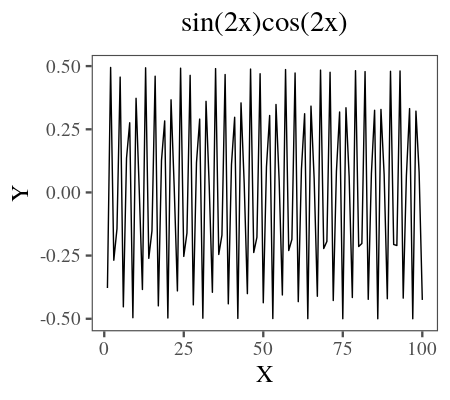
\includegraphics[width=.45\linewidth]{Figures/plotsincos.png}
	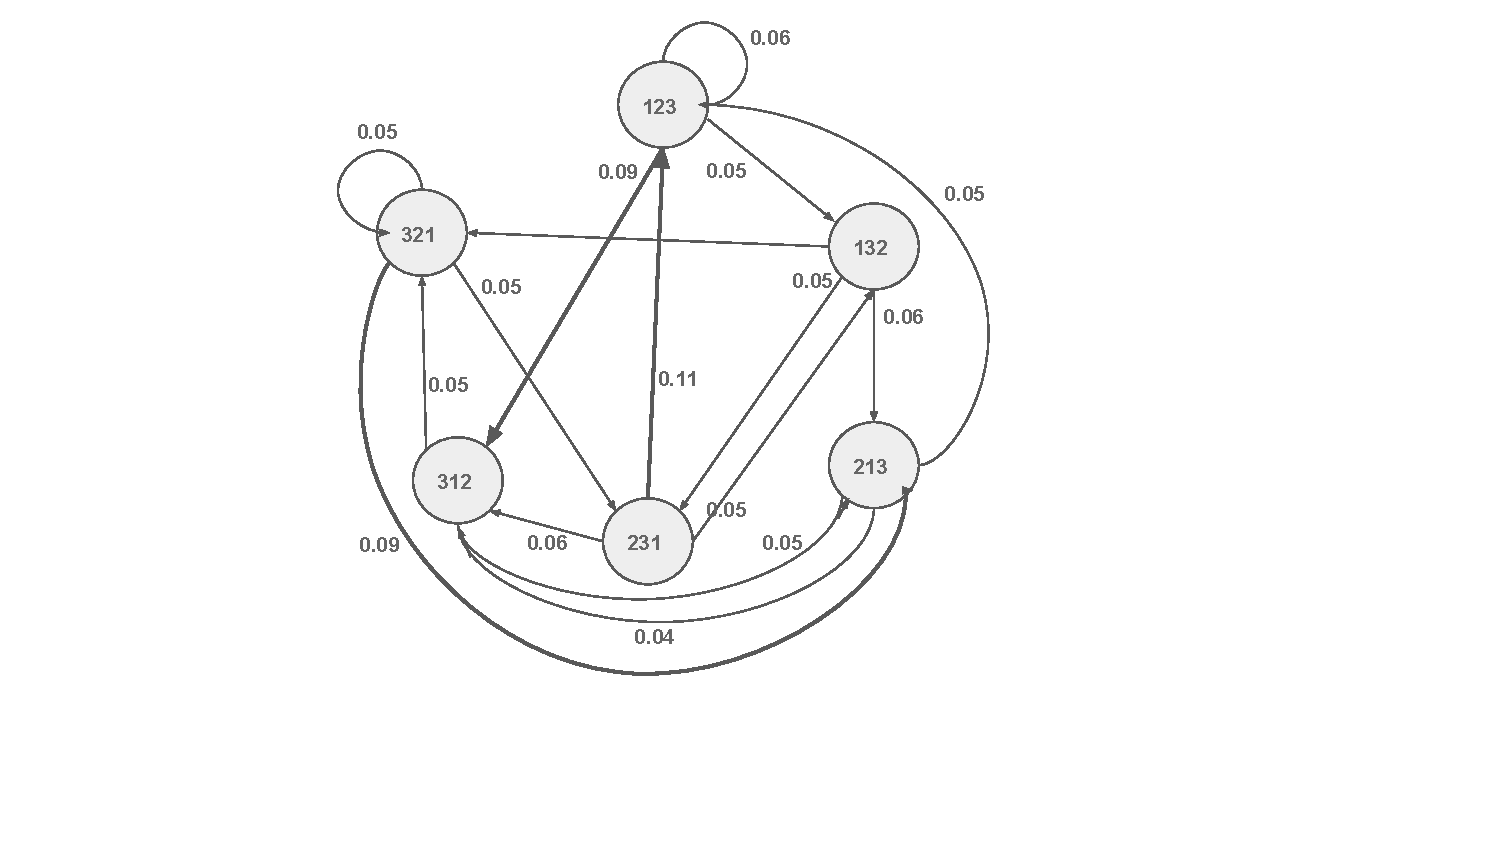
\includegraphics[width=.4\linewidth]{Figures/graph.pdf}
	\caption{Example of (a) the first 100 samples of the $sin (2x) \cdot cos (2x)$ series and (b) the WATG for the series with $D = 3$ and $\tau = 1$}\label{fig:series}
\end{figure} 

\subsection{Information-Theoretic Descriptors}\label{HC}

Entropy measures the disorder or unpredictability of a system characterized by a probability measure $\mathbb{P}$.

Let $\mathbb{P} = \{p_{(\widetilde\pi^D_1, \widetilde\pi^D_1)}, p_{(\widetilde\pi^D_1, \widetilde\pi^D_2)}, \dots, p_{(\widetilde\pi^D_{D!}, \widetilde\pi^D_{D!})} \} = \{p_1,\dots,p_{D!^2}\}$ be the probability distribution taken from the time series weighted amplitude transition graph $\mathbb{X}$.
The normalized Shannon entropy is given by:	
\begin{equation}
H(\mathbb{P}) = -\frac1{2\log D!}\sum_{\ell=1}^{D!^2} p_{\ell} \log p_{\ell} .
\label{eq:Entropia}
\end{equation}

The ability of the entropy to capture system properties is limited, so it is necessary to use it in conjunction with other des\-criptors to perform a more complete analysis.
Other interesting measures are distances between the $\mathbb{P}$ probability function and a probability measure that describes a non-informative process, typically the uniform distribution.

The Jensen-Shannon distance to the uniform distribution $\mathbb{U} = (\frac{1}{D!^2}, \dots, \frac{1}{D!^2})$ is a measure of how similar the underlying dynamics are to a process without information; it is calculated as:
\begin{equation}
Q'(\mathbb{P}, \mathbb{U}) = \sum_{\ell=1}^{D!^2} \Big(p_\ell \log\frac{p_\ell}{u_\ell} +
u_\ell \log\frac{u_\ell}{p_\ell}
\Big).
\end{equation}
This quantity is also called ``disequilibrium.''
The normalized disequilibrium is $ Q=Q'/\max\{Q'\}$.

Conversely to entropy, statistical complexity seeks to find interaction and dependence structures among the elements of a given series, being an extremely important factor in the study of dynamic systems.

The Statistical Complexity is then defined as~\cite{Lamberti2004}:
\begin{equation}
C(\mathbb{P}, \mathbb{U}) = H(\mathbb{P}) Q(\mathbb{P}, \mathbb{U}).
\end{equation}

In our analysis, each time series can then be described by a point $(H(\mathbb{P}), C(\mathbb{P}, \mathbb{U}))$.
The set of all pairs $(H(\mathbb{P}), C(\mathbb{P}, \mathbb{U}))$ for any time series described by patterns of length $D$ lies in a compact subset of $\mathbbm R^2$: the Entropy-Complexity plane. 

Through such a tool it is possible to discover the nature of the series, determining if it corresponds to a chaotic (or other deterministic dynamics) or stochastic sequences.

\section{TEXTURAL CLASSIFICATION OF SAR REGIONS}\label{SAR}

Widely used in recognizing geographical features and patterns, synthetic aperture radar (SAR) images are rich in texture information.
For this analysis, we used the HH intensity band of three different region SAR images with uninhabited aerial vehicle (UAVSAR) SAR data, which provide fully polarimetric SAR observations:
\begin{itemize}
	\item Sierra del Lacandon National Park, Guatemala (acquired on April 10, 2015)\footnote{\protect{\url{https://uavsar.jpl.nasa.gov/cgi-bin/product.pl?jobName=Lacand_30202_15043_006_150410_L090_CX_01\#dados}}};
	\item Cape Canaveral Ocean Regions (acquired on September 22, 2016);
	\item Urban area of the city of Munich, Germany (acquired on June 5, 2015)\footnote{\protect{\url{https://uavsar.jpl.nasa.gov/cgi-bin/product.pl?jobName=munich_19417_15088_002_150605_L090_CX_01\#data}}}.
\end{itemize}

We used $160$ samples of size $128\times128$, with the following configuration:
$40$ samples from Guatemalan forest regions;
$80$ samples from the oceanic regions of Cape Canaveral, where they were divided into two types that have distinct contrast information; and
$40$ samples of urban regions of the city of Munich.
Figure ~\ref{fig:RegionsSAR} shows examples of each of them.

\begin{figure}[hbt]
	\centering
	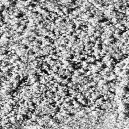
\includegraphics[width=.23\linewidth]{Figures/guatemalaflorest}
	
\includegraphics[width=.23\linewidth]{Figures/Cape1}
	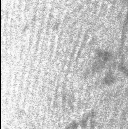
\includegraphics[width=.23\linewidth]{Figures/Cape2}
	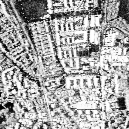
\includegraphics[width=.23\linewidth]{Figures/munichUrban}	
	\caption{Types of regions analyzed: Forest, Sea Type~1, Sea Type~2, and Urban.}\label{fig:RegionsSAR}
\end{figure} 

Since the symbolization process is invariant to monotonous transformations and resistant to contamination effects, contrast chan\-ges are not capable of causing changes in the final results obtained by the descriptors.
Thus, the different types of oceanic regions considered in this work were studied as a single more general class.

%Data resulting from remote sensing have a peculiar feature that justifies the application in this article:
%The intensities of an image and hence the amplitude difference in the data classes depend on the properties of the target we are analyzing due to the backscatter properties.
%Thus, urban targets are those that usually give the highest returns, followed by forests, and finally, water bodies, as can be seen in the figure~\ref{fig:AmplitudeSAR}.

%Therefore, in this paper we aim to represent, through the weighted amplitude transition graph, to model this amplitude difference in the probability distribution of our data.
%The analysis methodology proposed and applied to the texture data set SAR can be seen in the figure~\ref{fig:WATG}.

Figure~\ref{fig:AmplitudeSAR} shows examples of forest, sea and urban samples as time series, after the linearization process.

\begin{figure}[hbt]
	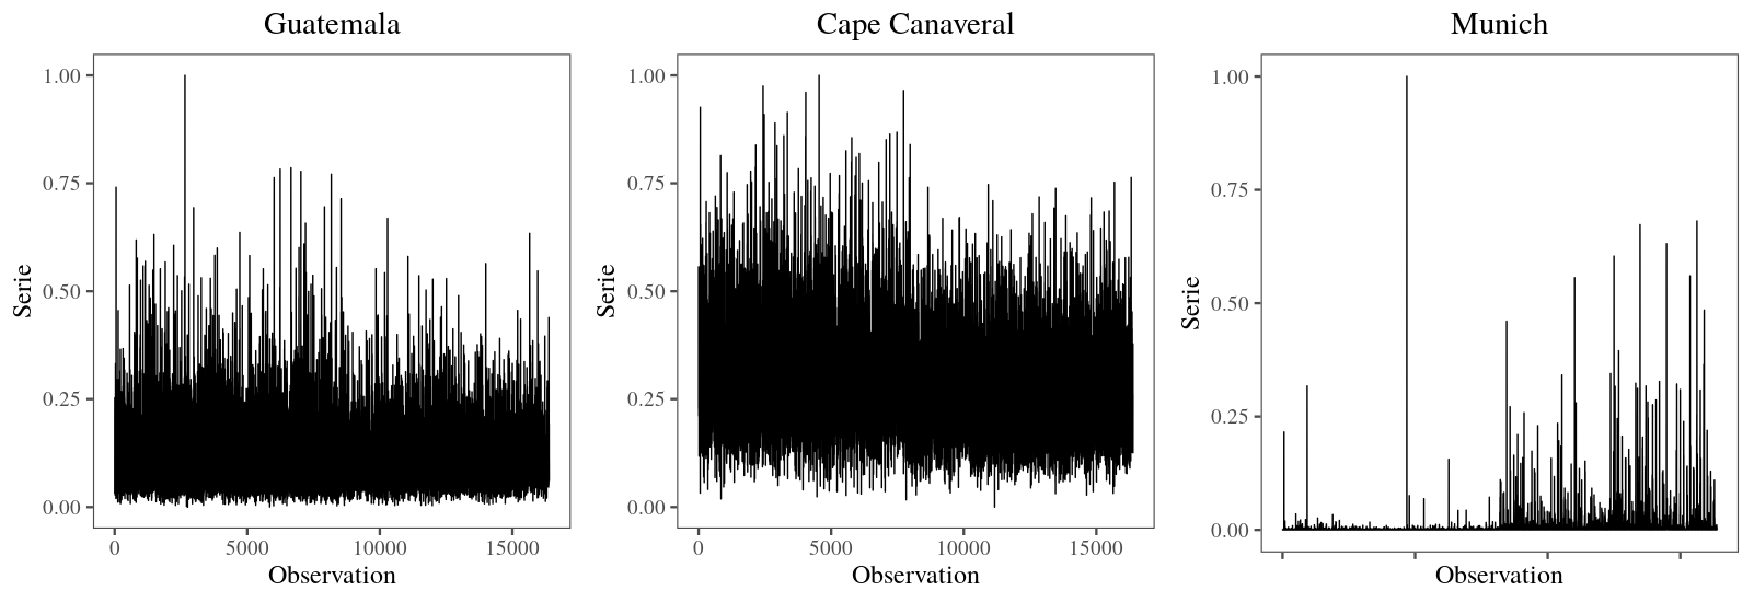
\includegraphics[width=\columnwidth]{Figures/SAR_signal.pdf}
	\caption{Analysis of the amplitude of the different types of regions: (a) Oceanic Region; (b) Forest Regions and (c) Urban Regions}
	\label{fig:AmplitudeSAR}
\end{figure}

%After linearizing the textures using the Hilbert curve, we used the sliding window technique to obtain our symbols, thus:
%\begin{equation}
%\mathbb{X}_t^{m,\tau} = (x_{t}, x_{t+\tau},\ldots, x_{t+(m-2)\tau} ,x_{t+(m-1)\tau}).
%\end{equation}

As we can see in Figure~\ref{fig:D3T1}, when we apply small delay and dimension values (the best result was obtained when $D = 3$ and $\tau = 1$) with WATG, in urban region data, we obtained a probability distribution with few extreme values, representing the transitions of the maximum values of the series.
On the other hand, oceanic and forest regions have as their main discriminating descriptor the statistical complexity that portrays the degree of temporal dependence structure between the symbols and consequently between the pixel intensity values.

Figure~\ref{fig:Regions} shows the results for several dimension values $m$ and delays $\tau$.
Since such values inform us of intrinsic characteristics of the dynamics of the series in their specific domains, inadequate values may hide this kind of knowledge about the data, and this analysis step is extremely crucial.

As shown in Figure~\ref{fig:Regions}, class discrimination decreases with $\tau$, which means that there is a loss of effect from the peak values found in the series, thus making a better distinction between classes when we have $\tau = 1$.
As WATG captures amplitude differences between different time series, when the values of the $\tau$ scale increase, well-distributed weight plots are formed, thus obtaining increasing entropy values.
On the other hand, as we increase $D$, the granularity of the information increases, capturing more spatial dependence structures in the data and, consequently, acquiring greater statistical complexity.
As can be seen in the Figure.~\ref{fig:Regions} There is a relationship between the dimension variable of ordinal patterns and the discrimination between the analyzed regions that presents its best result for $D = 3$.
On the other hand, when we have D = 6, textures acquire a lower entropy value and become harder to distinguish.

\begin{figure}[hbt]
	\centering
	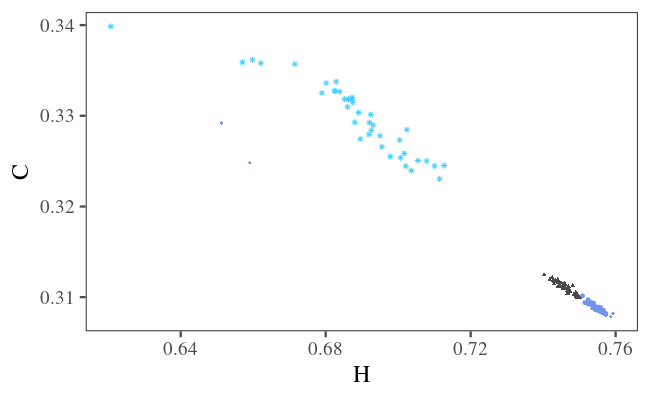
\includegraphics[width=0.9\columnwidth]{Figures/transitionGraphD3t1.png}
	\caption{Location of Guatemala (Black), Cape Canaveral (Blue) and Munich (Violet) in the $H \times C$ plane. Defaults were calculated with $D = 3$ and $\tau = 1$.}
	\label{fig:D3T1}
\end{figure}


\begin{sidewaysfigure*}
	\centering
	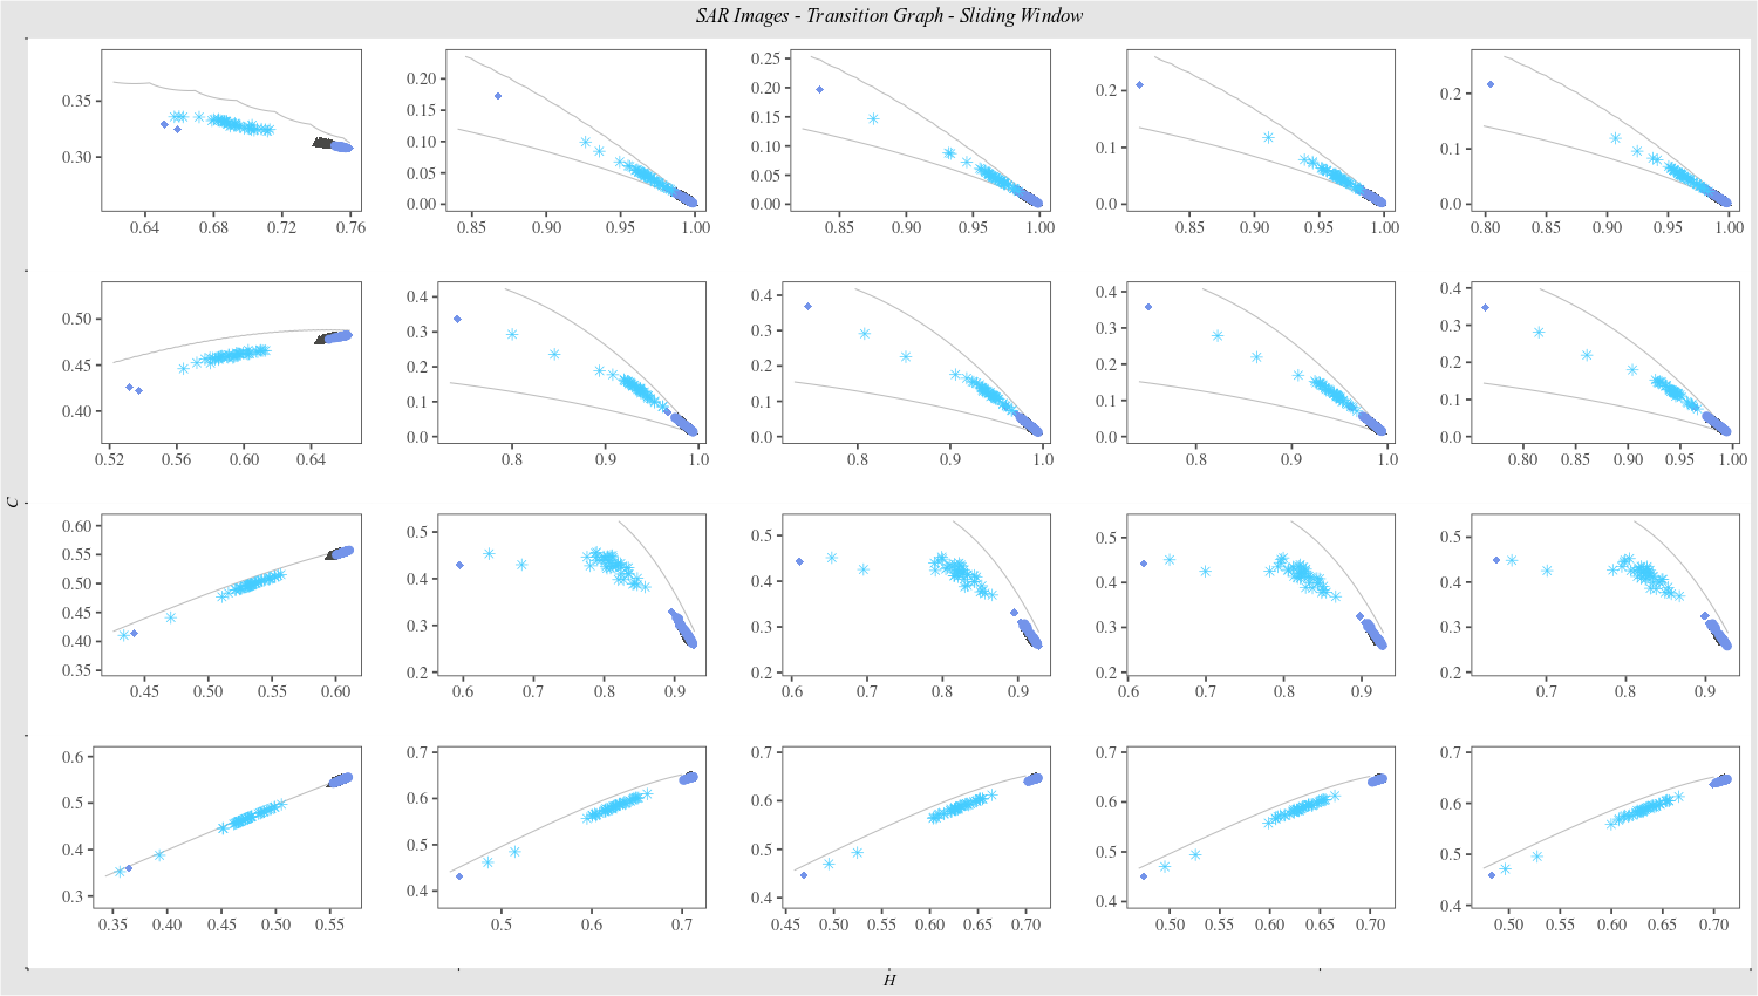
\includegraphics[width=1.05\textwidth]{Figures/transitionGraphHilbert.pdf}
	\caption{Characterization resulting from the application of the \texttt{Hilbert curve} in WATG on textures of different regions: Guatemala (Black), Cape Canaveral (Blue) and Munich (violet). Charts evolve horizontally according to the $m$ dimension chosen and vertically with the delay $\tau$}
	\label{fig:Regions}
\end{sidewaysfigure*}


\section{CONCLUSION}\label{Conclusion}

We proposed a new weighting technique in the formation of Ordinal Pattern Transition Graphs.
The edge weights are proportional to the amplitude variations during the transitions.
%Thus, the closer the entropy $\mathbb{H}$ is to $0$ the more uniform the probability distribution $\mathbb{P}$ will be, informing us that the series does not have large amplitude variances.
%However, if a series has a low amplitude but has large variations (peaks) over time, WATG will be able to infer such behavior by placing a greater weight on these transitions, making the entropy $\mathbb{H}$ approach $1$.

To test the proposed technique we performed the characterization of different regions in textures of SAR images.

As a result, in addition to perfectly separating urban areas from the others analyzed by entropy values, we are still able to differentiate oceanic and forest areas through their different values of statistical complexity, which informs us of the degree of temporal dependence between their elements.

\section{SOURCE CODE AVAILABILITY}

The source code generated during the current study are available in the \textit{SAR-WATG} repository, \url{https://github.com/EduardaChagas/SAR-WATG}.

\bibliographystyle{isprs}
\bibliography{../../Common/references.bib}

\section*{ACKNOWLEDGEMENTS}\label{ACKNOWLEDGEMENTS}

This work was partially funded by the Coordination for the Improvement of Higher Education Personnel (CAPES) and National Council for Scientific and Technological Development (CNPq).


\end{document}